\subsection{Results} \label{Sec:results}
\headbf{Effectiveness (RQ1)} \figref{assertionTypeFaultDetec} depicts the fault detection rate achieved by (1) \tool, (2) explicit assertions when included individually, and (3) explicit assertions in conjunction with either implicit assertions or (4) candidate assertions. The number on each bar represent the number of faults detected by the corresponding assertion types. As shown in \figref{assertionTypeFaultDetec}, \tool detects on average 62\% of the total faults (ranges from 42-84\%).
The percentage of faults revealed by including only explicit assertions is always less than the ones that are detected through the combination of explicit with either implicit assertions or candidate assertions. This indicates that implicit as well as candidate assertions are essential entities in improving the fault finding capability of \tool. By eliminating implicit and candidate assertions, fault detection rate drops by 27\% on average and up to 31\% for the EnterpriseStore application (ID 2).

\figref{assertionTypeFaultDetec} shows that the improvement brought by implicit assertions is 8\% on average, however, when candidate assertions are included fault detection rate is increased by 21\% on average. This indicates that candidate assertions play a more prominent role in increasing the number of faults detected by \tool in comparison with implicit assertions. Not surprisingly, explicit assertions contribute the most among the other assertion types generated by \tool. Explicit assertions detect 73\% of the total faults on average (ranges from 69-77\%). These assertions are derived directly from the DOM-based oracles written by the developer of the application who has a deep knowledge of the application's behaviour. Therefore, it is expected that code-level assertions derived directly from such oracles have the highest impact on fault finding capability of our tool.        

\begin{figure}[!t]
  \centering
  \includegraphics[width=1\hsize]{r-scripts/assertionTypeFaultDetec}
  \vspace{-0.18in} 
  \mycaption{Fault detection rate using different types of generated assertions.}
  \vspace{-0.1in} 
  \label{Fig:assertionTypeFaultDetec}
 
\end{figure}

\headbf{Comparison with human-written DOM-based Assertions (RQ2)}

\begin{figure}[!t]
  \centering
  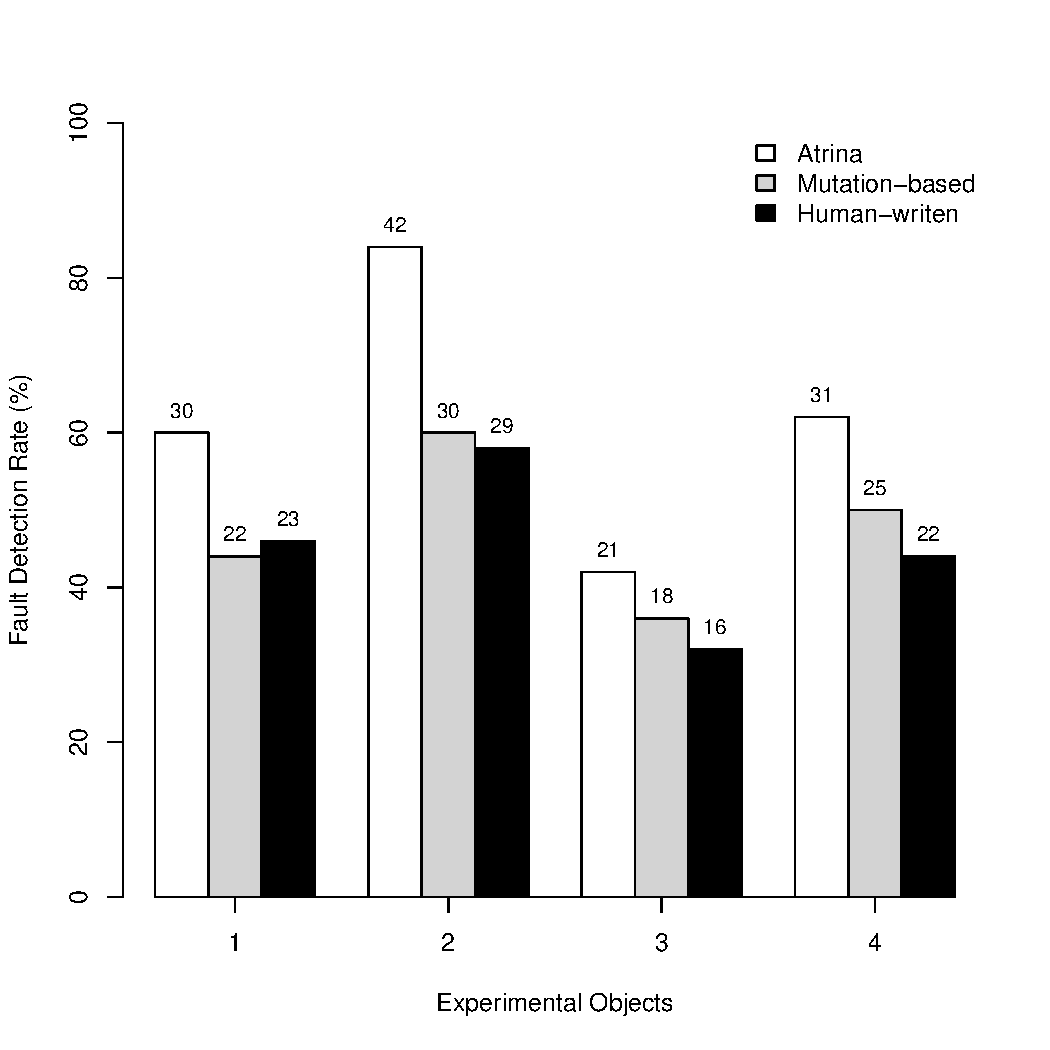
\includegraphics[width=1\hsize]{r-scripts/barplot-faultDetectionRate}
  \vspace{-0.18in}   
  \mycaption{Fault finding capability.}
  \vspace{-0.1in} 
  \label{Fig:faultDetectionRate}

\end{figure}

\headbf{Accuracy (RQ3)}
\begin{table}
        \caption{Accuracy achieved by \tool.} \label{Table:accuracyTable}        
{\scriptsize
\centering
%    \begin{center}
       
      %  \subtable[Experimental subjects and the corresponding exploration data]
            {
           \begin{tabular}{l|l|l|l|l|l} \hline
\theadturn{ID} &\theadturn{\# TP} &\theadturn{\# FP} &\theadturn{\# FN} &\theadturn{Precision (\%)} &\theadturn{Recall (\%)}  \\  \hline 

1  & 174 & 0 & 0 & 100 & 100    \\ \hline
           
2 & 861 & 18 & 162 & 98 & 84  \\ \hline

3 & 193 & 0 & 0 & 100 & 100  \\ \hline

4 & 1446 & 29 & 385 & 98 & 79 \\ \hline

\hline\end{tabular}
            }

%\end{center}
}
%\vspace{-0.2in} 
\end{table}
\headbf{Comparison with Mutation-based Assertion Generation (RQ4)}



